%%% Local Variables:
%%% mode: japanese-latex
%%% TeX-engine: uptex
%%% TeX-master: "okuda-master-thesis"
%%% TeX-PDF-mode: t
%%% TeX-PDF-from-DVI: "Dvipdfmx"
%%% End:

\newcommand*\ccircled[4]{\tikz[baseline=(char.base)]{
    \node[shape=circle, fill=#2, draw=#3, text=#4, inner sep=1pt] (char) {#1};}}
\newcommand{\cnum}[1]{\ccircled{#1}{MediumTurquoise!40}{MediumTurquoise!40}{black}}

\subsection{設定と$\ha$射影の定義}
本論文の基本的な設定は次のとおりであり,この他に必要な条件は都度明示することとする.

\begin{nttdef}\label{nttdef:fund}
  \leavevmode\vspace{-1em}
  \begin{itemize}
  \item $\nat,\real, \cpx,\quat$をそれぞれ0以上の整数全体,実数全体,複素数全体,四元数全体の集合とする.
  \item $G$を非コンパクト実線型簡約Lie 群とし,$H$を$G$の非コンパクトかつ連結成分有限個の閉部分群で,$G$のCartan対合$\Theta$に対して$\Theta H = H$なるものとする.

    % この定義は\cite[(2.6.1)]{kob89}に連結成分有限個の仮定を付け加えたものであるが,\cite[Definition-Lemma 2.6]{kob89}より.本論文ではこのような$H$を$G$の簡約な部分群と呼ぶことにする.
  \item $\ge \defeq \Lie G,\; \ha \defeq \Lie H$とし,$\ge = \ka\oplus \pe$を $\theta \defeq d\Theta$ によるCartan分解とする.
  \item $\ze(\ha)\defeq \{Y\in \ha\mid [Y,\ha] = \{0\} \} $とする.
  \item $e$を$G$の単位元とし,$o_K \defeq eK\in G/K$とする.
  \item $\lyama{-},{-} \ryama$を,$\ge$上の$G$-不変な非退化対称双線型形式で,$\ka$上負定値,$\pe$上正定値で$\ka$と$ \pe$が直交するものとする.
  \item $\per{\ha}\ \defeq \{W\in \ge\mid \lyama W, \ha\ryama = \{0\}\} $とする.
  \item $X\in \pe$に対し,ベクトル空間としての分解$\pe =( \ha\cap \pe)\oplus(\per{\ha}\cap \pe) $に対応した分解を$X = X_1 + X_2 $,$X_1 \in \ha\cap \pe$,$X_2\in \per{\ha}\cap \pe$とする.
  \item Riemann多様体$M$を$M$上の任意の2点に対しその2点をつなぐ一意的な測地線が存在するものとし,$d_M $を$M$上のRiemann計量から定まる距離とする.相異なる3点$p,q,r \in M$に対し,
    \begin{itemize}
    \item $\gamma_{p,q}\colon [0, d_{M}(p,q)] \to M$を,$\gamma(0) =  p$,$\gamma(d_{M}(p,q)) = q $なるunit speedの測地線とする.
    \item $\measuredangle_{p}(q, r)$を$\gamma_{p,q} $と$\gamma_{p,r} $が$p$においてなす角とする.
    \end{itemize}
  \end{itemize}  
\end{nttdef}

以下の\Cref{thm:kob89-lem6.1}を用いて,$X\in \pe$に対し,
\begin{align*}
{(Y(X), Z(X))\defeq \inv{\pi}(e^X\cdot o_K)\in (\ha\cap\pe)\oplus (\per{\ha}\cap \pe)}
\end{align*}
と定義し,本稿ではこの$Y\colon \pe\to \ha\cap \pe $を``$\ha$射影''と呼ぶことにする.

\begin{thm}(\cite[Lemma~6.1]{kob89})\label{thm:kob89-lem6.1}
  $H$を$G$の非コンパクトかつ連結成分有限個の閉部分群で,$G$のCartan対合$\Theta$に対して$\Theta H = H$なるものとする.このとき
  \begin{align*}
    \pi\colon  (\ha\cap\pe)\oplus (\per{\ha}\cap \pe) \ni (Y, Z)\mapsto e^{Y}e^{Z}\cdot o_K \in G/K
  \end{align*}
  は上への微分同相である.
\end{thm}


ここで,$Y(\real X) $の有界性について,次の\Cref{prob:1121}が小林俊行氏によって提起された.


\begin{prob}(小林俊行氏による)\label{prob:1121}
  ${\pe_{H,\bdd}\defeq \{X\in \pe\mid Y(\real X)\text{ が } \ha\cap \pe \text{ の有界集合である.}  \}}  $と定めるとき,
  \begin{enumerate}
  \item $G$が実線型半単純Lie群ならば$\pe\setminus\pe_{H,\bdd} $はLebesgue測度に対して測度0であるか?
  \item $X\in \pe_{H,\bdd}$であることと次の\Cref{cond:0117}は同値であるか?
    \begin{cond}\label{cond:0117}
      $X\in \pe$は次のいずれかを満たす.
      \begin{itemize}
      \item[\ccircled{1}{MediumTurquoise!40}{MediumTurquoise!40}{black}] $X\in \per{\ha}\cap\pe $
      \item[\ccircled{2}{MediumTurquoise!40}{MediumTurquoise!40}{black}] $[X_1, X_2 ] \neq 0$かつ$X\in \ge_{s}' $である.
      \item[\ccircled{3}{MediumTurquoise!40}{MediumTurquoise!40}{black}] $[X_1, X_2 ] \neq 0$かつ$\pe\cap \ze(\ge') \nsubset \ha $である.
      \end{itemize}
      ただし$\ge' $は$\ha$と$X$により生成される$\ge$の部分Lie環とする.$\ge' $は$\theta$不変であるから$\ge_{s}' \defeq [\ge', \ge'] $とすると$\ge'  = \ze(\ge') \oplus \ge_{s}' $である.
    \end{cond}
  \end{enumerate}
\end{prob}

\Cref{cond:0117}で定めた$\ge'$の元$X$に対して次の記法を導入する.
\begin{defi}
  $X\in \ge' $に対し,ベクトル空間としての分解$\ge' = \ze(\ge') \oplus \ge_{s}' $に対応した分解を$X = X_c + X_s $,$X_c \in \ze(\ge')$,$X_s\in \ge_{s}'$とする.
\end{defi}

\subsection{\Cref{prob:1121}の基本性質}
\Cref{prob:1121}についての基本的な事項を挙げる.

\begin{prop}\label{lem:basic-prob}
  \leavevmode\vspace{-1em}
  \begin{enumerate}[label=\textbf{\arabic*.}]
  % \item \Cref{prob:1121}において,2が成り立つならば1が成り立つ.
  \item $X\in \pe_{H,\bdd} $ならば$X$は\Cref{cond:0117}を満たす.
  \item $X \in \pe $が$X_1 = 0$を満たすならば$X\in \pe_{H,\bdd} $である.
  \item $G$が実階数1ならば,$X\in\pe$が\Cref{cond:0117}を満たすことと$X\in \{0\}\cup \pe\setminus\ha $であることは同値である.
  \end{enumerate}
\end{prop}

いくつか補題を用意してから\Cref{lem:basic-prob}を示す.以下$\ha_s\defeq \ge_{s}'\cap\ha $とする.
\begin{lem}\label{lem:0117-perp}
  $\pe\cap \ze(\ge')\subset \ha $ならば$\ge'_s\cap\pe $における$\ha_s\cap \pe$の直交補空間は$\per{\ha}\cap\pe $に含まれる.
\end{lem}
\begin{npfwn}[\Cref{lem:0117-perp}]
  $\ha\subset \ge' $であり,両者とも$\theta$不変であるから,
  \begin{align}
    \ha &= (\ge'_s\cap \ha)\oplus (\ze(\ge')\cap\ha )\notag \\
        &= \ha_s\oplus (\ze(\ge')\cap\ha\cap\ka )\oplus (\ze(\ge')\cap\ha\cap\pe ) \notag\\
        &= \ha_s\oplus (\ze(\ge')\cap\ha\cap\ka )\oplus (\ze(\ge')\cap\pe ) \label{eq:0117-perp}
  \end{align}
  である.最後の等式には$\pe\cap \ze(\ge')\subset \ha $を用いた.

  任意の$X\in \per{\ha_s}\cap \ge'_s\cap\pe $と$Y\in \ha\cap\pe $の元を取る.$Y$を\Cref{eq:0117-perp}の分解に対応して$Y = Y_s + Y_{\ka} + Y_{c} $と分解する.
  
  $X\in\per{\ha_s}\cap \pe $と$\ka\perp\pe $であるから
  \begin{align*}
    \lyama X, Y\ryama &= \lyama X, Y_s + Y_{\ka} + Y_{c}\ryama = \lyama X,   Y_{c}\ryama
  \end{align*}
  である.$X\in \ge_{s}' = [\ge', \ge'] $より,ある$T,\ S\in \ge'$が存在して$X = [T, S] $である.$\lyama {-}, {-}\ryama $は$G$不変であるから
  \begin{align}
    \lyama X, Y\ryama &= \lyama X,   Y_{c}\ryama = \lyama [T, S],   Y_{c}\ryama = -\lyama S,   [T, Y_{c}]\ryama\label{eq:0117-perp-2}
  \end{align}
  である.ここで$Y_c\in \ze(\ge') $より$[T, Y_c ]= 0$であるから\Cref{eq:0117-perp-2}の左辺は0となり,\Cref{lem:0117-perp}の主張を得る.
\end{npfwn}

\begin{lem}\label{lem:0117-closed}
  $G_s $を$\ge_{s}' $の$G$における解析的部分群,$H_s $を$\ha_s $の$G$における解析的部分群とする.このとき$G_s$,$H_s$はともに$G$の閉部分群であり,$\Theta H_s = H_s $である.
\end{lem}
\begin{npfwn}[\Cref{lem:0117-closed}]
  $\ge_s' $,$\ha_s $は実半単純Lie環であり,$G$は線型Lie群であるから,後述の\Cref{thm:yos38}より$G_s$,$H_s$は$G$の閉部分群である.

  $\ge_{s}'$と$\ha $はともに$\theta$不変より$\theta \ha_s = \ha_s $であるから\Cref{lem:0117-closed},特に$H_s$の非コンパクト性を除いて\Cref{nttdef:fund}の条件すべてが成り立つ.
\end{npfwn}

\begin{defi}

  \Cref{lem:0117-perp}の仮定のもとで$G_s\supset H_s$,$X\in \pe\cap\ge_{s}' $に対し,$Y_s(X)\in \ha_s\cap\pe \subset \ha\cap \pe $と$Z_s(X)\in \per{\ha_s}\cap \pe \subset \per{\ha}\cap \pe $を次のように定める.
  
  $H_s $が非コンパクトならば\Cref{lem:0117-closed}により,$K_s\defeq G_s\cap K $,$(G_s, H_s, G_s/K_s) $に対して\Cref{thm:kob89-lem6.1}を用いて,$X\in \pe\cap\ge_{s}' $に対し
  \begin{align*}
    {(Y_s(X), Z_s(X))\defeq \inv{\pi}(e^X\cdot o_K)\in (\ha_s\cap\pe)\oplus (\per{\ha_s}\cap \pe)}
  \end{align*}
  と定義する.


  $H_s $がコンパクトな場合は$\ha_s = \theta \ha_s$より$\ha_s\subset \ka $,したがって$H_s\subset K $であるから,$X\in \pe\cap\ge_{s}' $に対し,$Y_s(X) = 0 $,$Z_s(X) = X $と定義する.
\end{defi}

\begin{lem}\label{lem:0117-decomp}
  \Cref{lem:0117-perp}の仮定のもとで任意の$X = X_c + X_s \in \ge'\cap\pe $に対し$Y(X) = X_c + Y_s(X_s) $である.
\end{lem}
\begin{npfwn}[\Cref{lem:0117-decomp}]

  \leavevmode
  \begin{itembox}[l]{補助補題1}
    指数写像によって$G_s/K_s \simeq \ge_s'\cap \pe $であるから,任意の$X, X'\in \ge_{s}'\cap \pe $に対し,ある$\tilde{X}\in \ge_s'\cap \pe$が存在して,$e^{X}e^{X'}K_s = e^{\tilde{X}}K_s  $である.$K_s\subset K $であるから$e^{X}e^{X'}\cdot o_K = e^{\tilde{X}}\cdot o_K $である.
  \end{itembox}
  
  
  \begin{itembox}[l]{補助補題2}
    $X,\ X'\in \ge'\cap\pe $に対し$\exp(X_c)\exp(X_s)\cdot o_K = \exp(X_c')\exp(X_s')\cdot o_K $ならば$\exp(X_c-X_c'+X_s)\cdot o_K = \exp(X_s')\cdot o_K $であることと$\ze(\ge')\cap \ge_s' = \{0\} $より$X_c = X_c' $,$\exp(X_s)\cdot o_K = \exp(X_s')\cdot o_K$である.
  \end{itembox}
  
  $Y(X)\in \ha\cap\pe\subset \ge' $,$Z(X)\in \per{\ha}\cap\pe\subset \ge' $より$Y(X) = Y(X)_c + Y(X)_s $,$Z(X) = Z(X)_c + Z(X)_s $,$Y(X)_c,\ Z(X)_c \in \ze(\ge')\cap\pe  $,$Y(X)_s,\ Z(X)_s\in \ha_s\cap\pe $と分解できる.

  このとき,$[X_c, X_s] = 0 $,$[X_c', X_s'] = 0$より$\exp(X)\cdot o_K = \exp(X_c)\exp(X_s)\cdot o_K $であるから
  \begin{align*}
    e^{X_c}e^{X_s}\cdot o_K &= e^{X}\cdot o_K \\
                            &= e^{Y(X)}e^{Z(X)}\cdot o_K\\
                            &= e^{Y(X)_c + Y(X)_s}e^{Z(X)_c + Z(X)_s}\cdot o_K\\
                            &= e^{Y(X)_c + Z(X)_c}e^{Y(X)_s}e^{Z(X)_s}\cdot o_K
  \end{align*}
  であるから,補助補題1と2より
  \begin{align}
    X_c &= Y(X)_c + Z(X)_c ,\label{eq:zensha} \\
    e^{X_s}\cdot o_K &= e^{Y(X)_s}e^{Z(X)_s}\cdot o_K\label{eq:kousha}
  \end{align}
  である.

  \Cref{eq:zensha}より$e^{X_c} \cdot o_K = e^{Y(X)_c}e^{Z(X)_c}\cdot o_K $であり,\Cref{lem:0117-perp}の仮定より$Y(X)_c \in \ha\cap \pe$,$  Z(X)_c \in \per{\ha}\cap \pe$であるから$Y(X_c) = Y(X)_c $を得る.さらに\Cref{lem:0117-perp}の仮定より$X_c\in \ze(\ge')\cap \pe\subset \ha \cap \pe $であるから$Y(X_c) = X_c = Y(X)_c $を得る.

  また\Cref{eq:kousha}と$Y_s$の定義より$Y_s(X_s) = Y(X)_s $を得る.

  以上より$Y(X) = Y(X)_c + Y(X)_s = Y(X_c) + Y_s(X_s) = X_c + Y_s(X_s) $を得,\Cref{lem:0117-decomp}が示された.
\end{npfwn}

\begin{npfwn}[\Cref{lem:basic-prob}]
  \leavevmode\vspace{-1em}
  \begin{enumerate}[label=\textbf{\arabic*.}]
  % \item % \redtext{次が測度0であることを示せば十分である.}\footnote{示せていません.}
    
  \item $X\in \pe$が\Cref{cond:0117}を満たさないとき,$X\in \pe\setminus\pe_{H,\bdd} $であることを示せば良い.
    
    $X\in \pe$が\Cref{cond:0117}の \cnum{1} を満たさないことから$X\in\pe\setminus\per{\ha} $である.

    $X\in \pe\setminus\per{\ha} $なる$X$に対し$[X_1,X_2] = 0$ならば$e^{tX_1}e^{tX_2}\cdot o_K = e^{t(X_1 + X_2)}\cdot o_K = e^{tX}\cdot o_K$である.したがって\Cref{thm:kob89-lem6.1}より$Y(tX) = tX_1 $,$Z(tX) = tX_2 $であることから$Y(\real X) = \real X_1 $となり,$X_1\neq 0$より$Y(\real X)$は有界集合とならない.つまり$X\nin\pe_{H,\bdd} $である.

    次に$X\in \pe\setminus \per{\ha} $かつ$[X_1,X_2] \neq 0$なる$X$を考える.

    このとき\Cref{cond:0117}の \cnum{2},\cnum{3} が成り立たないことから$X\nin \ge_{s}' $かつ$\pe\cap \ze(\ge')\subset \ha $である.このとき$X = X_c + X_s $に対し$X_c\neq 0$であるから\Cref{lem:0117-decomp}より$Y(\real X)$は非有界であり,$X\nin\pe_{H,\bdd} $である.

    % $\pe\cap \ze_{\ze(\ha)}(X) \neq \{0\} $なる$X$に対し,$0\neq W\in\pe\cap \ze_{\ze(\ha)}(X)\subset \ha\cap \pe $を任意に1つ取る.このとき$X_2 \defeq  X - \dfrac{\lyama X, W\ryama }{\lyama W, W\ryama}W \in \per{\ha}\cap \pe $であり,$[X, W] = 0 $ より$[X_2, W] = 0$である.よって$X_1 \defeq \dfrac{\lyama X, W\ryama }{\lyama W, W\ryama}W $とすると,任意の$t\in \real$に対し$e^{tX_1}e^{tX_2}\cdot o_K = e^{t(X_1 + X_2)}\cdot o_K = e^{tX}\cdot o_K $である.よって$Y(\real X) = \real X_1 $より$X\nin\pe_{H,\bdd} $である.

    以上より主張が従う.
  \item $X_1 = 0$であることと$ X\in \per{\ha}\cap\pe $であることが同値であり$X\in \per{\ha}\cap\pe $ならば\Cref{thm:kob89-lem6.1}より$Y(X) = 0 $であることから主張が従う.
  \item $G$が実階数1のときに$X\in \pe$に対して$X\in \{0\}\cup \pe\setminus \ha $であることと\Cref{cond:0117}を満たすことが同値であることを示せば良い.$G$の実階数が1かつ$H$が非コンパクトで$\ha = \theta\ha$であるから$\ha\cap\pe$は極大分裂可換部分代数である.

    $X\in(\ha\cap\pe)\setminus\{0\} $ならば\Cref{cond:0117}を満たさないことは明らかであるから,\Cref{cond:0117}を満たさないならば$X\in(\ha\cap\pe)\setminus\{0\} $であることを示せば良い.

    
    
    \Cref{cond:0117}を満たさない$X\in \pe$を任意に1つ固定する.\Cref{cond:0117}の \cnum{1} が成り立たないことから$X\in \pe\setminus\per{\ha}$である.また$X$は\Cref{cond:0117}の \cnum{2},\cnum{3} を満たさない.もし$[X_1, X_2] = 0 $ ならば$\ha\cap\pe$が極大分裂可換部分代数であることから$X\in\ha\cap \pe $であるから,$X\in \ha\setminus\{0\} $が言える.

    以上より$[X_1,X_2] \neq 0$かつ$X\in \pe\setminus\per{\ha}$なる$X$のみを考えれば十分である.このとき$X$は\Cref{cond:0117}の \cnum{2},\cnum{3} を満たさないことからさらに$X\nin \ge_{s}' $かつ$\pe\cap\ze(\ge')\subset \ha $である.$X  = X_c + X_s $に対し,前者より$X_c\neq 0 $を得る.後者より$X_c\in \pe\cap\ze(\ge')\subset \ze_{\ha\cap\pe}(X) $である.しかし$\ha\cap \pe$は極大分裂可換部分代数であるから,$X\nin\ha\setminus\{0\} $ならば$[X, \ha\cap\pe ] \neq  \{0\}$より,$0 = X_c \in \ze_{\ha\cap\pe}(X) $とならざるを得ない.これは$X_c\neq 0 $に矛盾するから$X \in \ha\setminus\{0\}  $である.
    
    以上の議論から\Cref{lem:basic-prob}が示された.
  \end{enumerate}  
\end{npfwn}

$Y(\real X) $の有界性は$k\in K$に対して$\Ad(k) $不変な性質である.具体的には\Cref{lem:1101}が成り立つ.
\begin{lem}\label{lem:1101}
  任意の$k\in K$,$X\in \pe$に対し,$X'\defeq \Ad(k)X $,$\ha'\defeq \Ad(k)\ha $とする.微分同相$\pi'\colon (\ha'\cap \pe)\oplus (\per{\ha'}\cap \pe)\ni (Y',Z')\mapsto e^{Y'}e^{Z'}\cdot o_K  $を用いて,$X'\in \pe$に対し,$(Y'(X'), Z'(X')) = \inv{\pi'}(e^{X'}\cdot o_K) $と定める.このとき$Y(\real X)$が有界であることと$ Y'(\real X') $が有界であることは同値である.
\end{lem}

\begin{npfwn}[\Cref{lem:1101}]
  主張は$(X,\ha) $と$(X',\ha')$に対して対称的であるから,$Y(\real X) $が有界ならば$Y'(\real X') $が有界であることのみを示せば十分である.

  任意に$r\in \real$を取る.定義より$e^{rX'}\cdot o_K = e^{Y'(r X')}e^{Z'(r X')}\cdot o_K  $であり,両辺に左から$\inv{k} $を掛けると,$e^{r X} = e^{\Ad(\inv{k})( Y'(r X'))}e^{\Ad(\inv{k})( Z'(r X'))}\cdot o_K  $を得る.$Y'(rX')\in \ha'\cap \pe $,$Z'(r X')\in \per{\ha'}\cap \pe $であるから$\Ad(\inv{k})(Y'(r X'))\in \ha\cap \pe $,$\Ad(\inv{k})(Z'(r X')) \in \per{\ha}\cap \pe $である.

  \Cref{thm:kob89-lem6.1}により$\pi$は微分同相であるから,任意の$r\in \real$に対して$\Ad(\inv{k})(Y'(r X')) = Y(rX)  $である.したがって$Y'(\real X) = \Ad(k)(Y(\real X))  $であり,$\Ad(k) $は有限次元空間の間の線型写像であるから有界性を保つ.

  以上から\Cref{lem:1101}が示された.  
\end{npfwn}


$Y(\real X) $の有界性を判定しようとする\Cref{prob:1121}と比較して$Z(\real X) $の有界性については次の定理が知られており,有界性の判定はLie環の言葉のみで行える.

\begin{thm}(\cite[Lemma~5.4]{kob97})\label{thm:kob97}
  $X\in \pe$に対し,$\norm{X}\geq \norm{Z(X)}\geq \norm{X} \sin\phi(X, \ha\cap\pe)$が成り立つ.ここに$\phi(X,\ha\cap \pe) $は$X$と$\ha\cap \pe$の0でない元が$\pe$においてなす角度の最小値${0\leq \phi(X,\ha\cap \pe) \leq \frac{\pi}{2}} $であり,$X\in \pe\setminus \ha $と$ \phi(X,\ha\cap \pe)\neq 0 $は同値である.
\end{thm}

\Cref{thm:kob97}より,$X\in \ha\cap\pe $であることと$Z(\real X) $が有界であることが同値である.


\subsection{\Cref{prob:1121}の観察: $G = \SU(1,1) $,$H = \SO(1,1) $の場合}

$G = \SU(1,1) $,$H = \SO(1,1) \defeq\lbig\{
\begin{pmatrix}
  \cosh t & \sinh t\\ \sinh t & \cosh t
\end{pmatrix}
\relmiddle| t\in \real \rbig\} $は\Cref{prob:1121}の肯定的な例である.具体的には$\pe_{H,\bdd} = \{0\}\cup \pe\setminus\ha $である.

\begin{prop}\label{prop:prob-eg}
  $G = \SU(1,1) $,$H = \SO(1,1) $のとき$\pe_{H,\bdd} = \{0\}\cup \pe\setminus\ha $である.
\end{prop}

% \bluetext{$\sulie(1,1) $のKilling形式と$r = \tanh t$の関係を明記せよ.}
\Cref{prop:prob-eg}を示すために補題を1つ用意する.
\begin{lem}\label{lem:riem-metric-su11}
  {\Poincare}円板${G/K =\{x+\sqrt{-1}y\mid  x^2 + y^2 < 1 \} }$の$\ge\defeq \sulie(1,1)$のKilling形式から定まるRiemann計量$g$は$ \dfrac{8(dx^2 + dy^2)}{(1 - x^2 - y^2)^2} $である.
\end{lem}

\begin{npfwn}[\Cref{lem:riem-metric-su11}]
  
  $\pe$の元を$G/K$上の左不変ベクトル場と同一視すると
  \begin{align*}
    X' &\defeq 
         \begin{pmatrix}
           0 & 1 \\ 1 & 0
         \end{pmatrix} = \dfrac{\del}{\del x},\\
    Y' &\defeq 
         \begin{pmatrix}
           0 & \sqrt{-1} \\ -\sqrt{-1} & 0
         \end{pmatrix} = \dfrac{\del}{\del y}
  \end{align*}
  である.$\ge$のKilling形式$B$から定まる$\pe$上のノルム$\norm{-} $に対して$\norm{X'}^2 = \norm{Y'}^2 = 8 $,$B(X', Y' ) = 0$であるから$0\in G/K =\{x+\sqrt{-1}y\mid x^2 + y^2 < 1 \}  $において主張が成り立つ.

  したがって$k_{\theta} \defeq \diag(e^{\sqrt{-1}\theta},e^{-\sqrt{-1}\theta}) $,$a_r\defeq
  \begin{pmatrix}
    \cosh r & \sinh r \\  \sinh r & \cosh r
  \end{pmatrix}
  $とすると,
  \begin{align*}
    &g(d\tau(k_{\theta/2}a_r)(d\tau(k_{-\theta/2})X'), d\tau(k_{\theta/2}a_r)(d\tau(k_{-\theta/2})X')) \\
    =&\ g (d\tau(k_{\theta/2}a_r)(d\tau(k_{-\theta/2})Y'), d\tau(k_{\theta/2}a_r)(d\tau(k_{-\theta/2})Y')) \\
    =&\ 8, \\
    &g(d\tau(k_{\theta/2}a_r)(d\tau(k_{-\theta/2})X'), d\tau(k_{\theta/2}a_r)(d\tau(k_{-\theta/2})Y'))  = 0
  \end{align*}
  なるような計量$g $がKilling形式から誘導される計量である.$g$が主張の形であることを示す (\Cref{fig:riem-metric-su11}参照).

  \begin{figure}[H]
    \centering
    % \raggedleft
    % \raggedrightp
    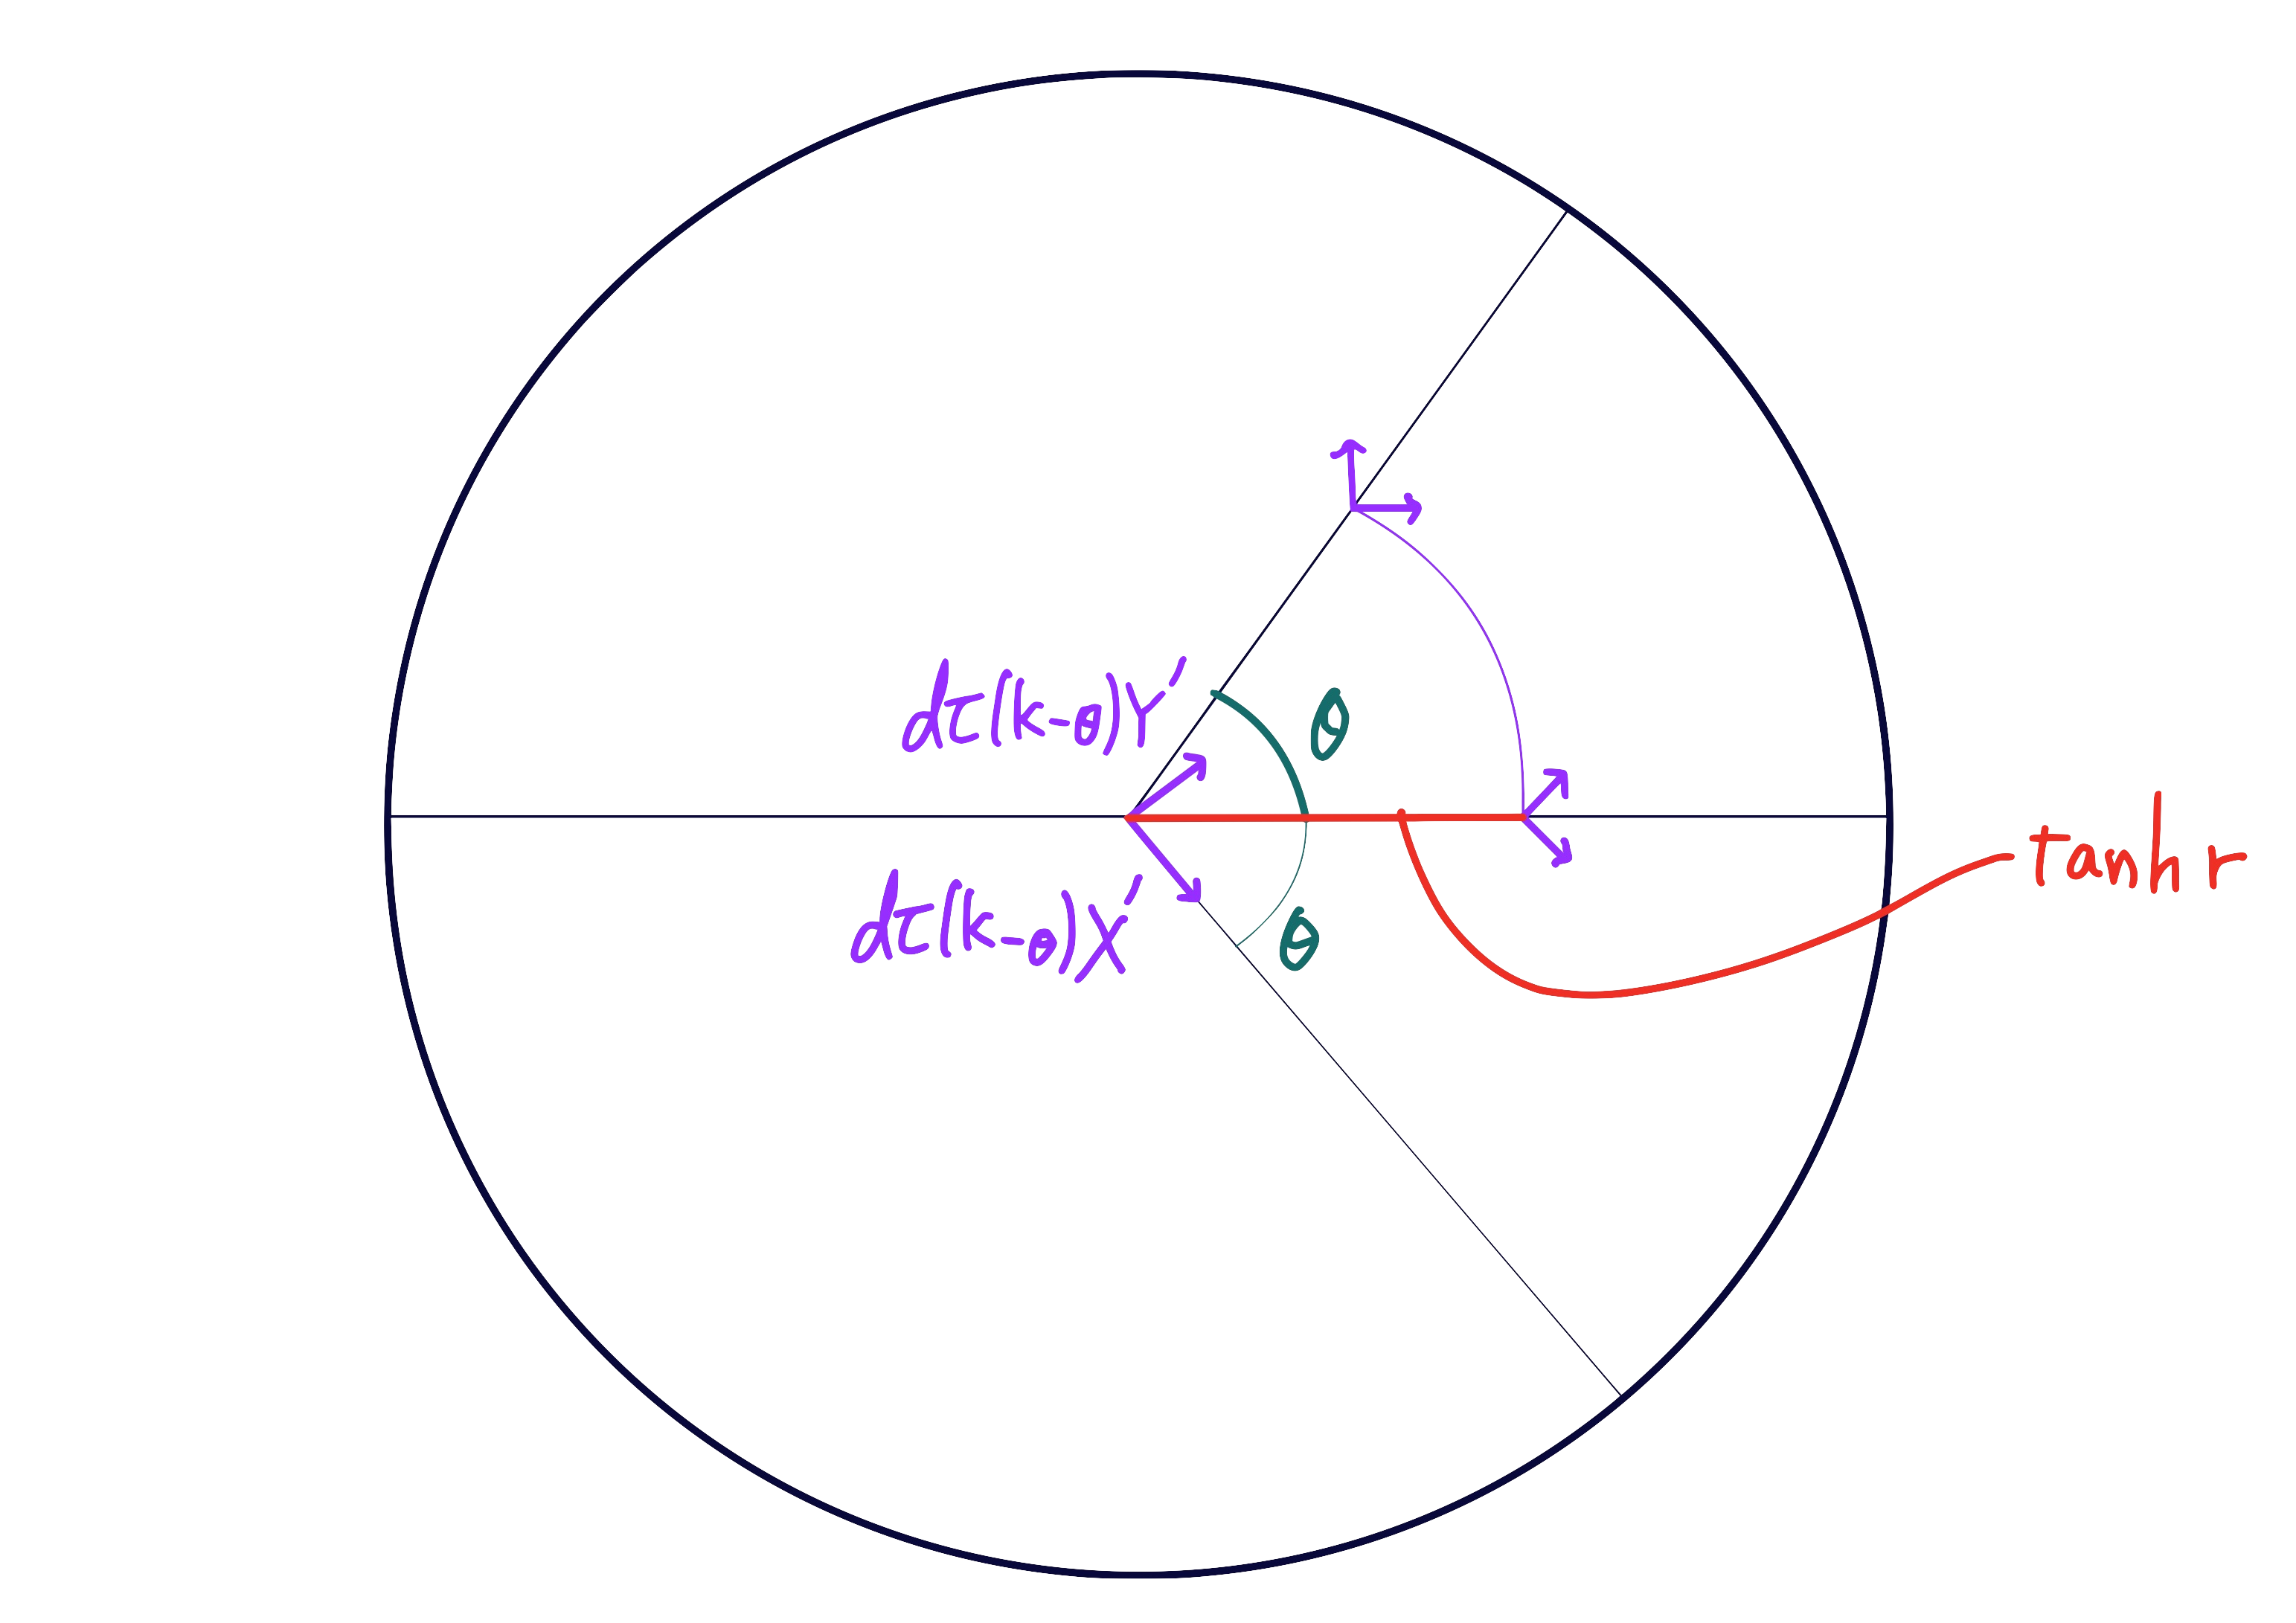
\includegraphics[scale=0.08]{../graph/riem-su11.png}
    % 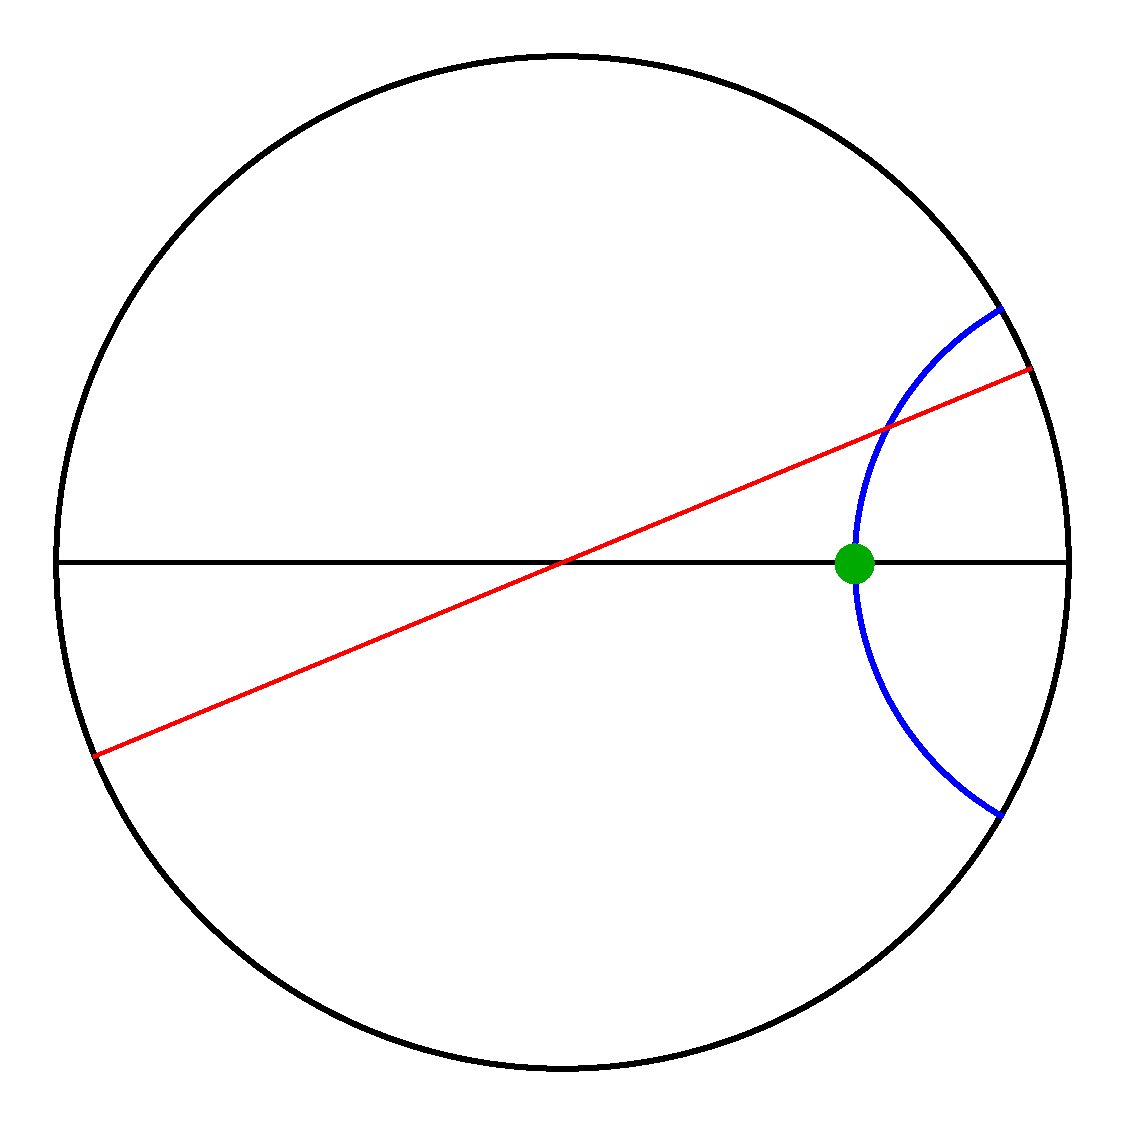
\includegraphics[scale=0.3]{../graph/y-and-z.pdf}
    \caption{}
    \label{fig:riem-metric-su11}
  \end{figure}


  $t = 0$での接ベクトルが$d\tau(k_{\theta/2}a_r)d\tau(k_{-\theta/2})X'$を与える曲線として
  \begin{align*}
    \gamma_x(t) \defeq  e^{\sqrt{-1} \theta}\dfrac{\cosh r\cdot e^{-\sqrt{-1}\theta} \tanh t + \sinh r }{\sinh r\cdot e^{-\sqrt{-1}\theta} \tanh t + \cosh r}
  \end{align*}
  が考えられるから
  \begin{align*}
    \lbig.\dfrac{d}{dt}\rbig|_{t=0}\gamma_x(t) = d\tau(k_{\theta/2}a_r)d\tau(k_{-\theta/2})X' = (1 - \tanh^2 r)\dfrac{\del}{\del x} = (1-x^2-y^2)\dfrac{\del}{\del x}
  \end{align*}
  である.

  同様に$t = 0$での接ベクトルが$d\tau(k_{\theta/2}a_r)d\tau(k_{-\theta/2})Y'$を与える曲線として
  \begin{align*}
    \gamma_y(t) \defeq  e^{\sqrt{-1} \theta}\dfrac{\cosh r\cdot e^{-\sqrt{-1}\theta}\sqrt{-1} \tanh t + \sinh r }{\sinh r\cdot e^{-\sqrt{-1}\theta}\sqrt{-1} \tanh t + \cosh r}
  \end{align*}
  が考えられるから
  \begin{align*}
    \lbig.\dfrac{d}{dt}\rbig|_{t=0}\gamma_y(t) = d\tau(k_{\theta/2}a_r)d\tau(k_{-\theta/2})Y' = (1 - \tanh^2 r)\dfrac{\del}{\del y} = (1-x^2-y^2)\dfrac{\del}{\del y}
  \end{align*}
  である.

  以上より$g  =  \dfrac{8(dx^2 + dy^2)}{(1 - x^2 - y^2)^2} $が得られる.
\end{npfwn}


\begin{npfwn}[\Cref{prop:prob-eg}]


  $k_{\theta} \defeq \diag(e^{\sqrt{-1}\theta},e^{-\sqrt{-1}\theta}) $,$X_{\theta} \defeq k_{\theta/2}
  \begin{pmatrix}
    0 & 1 \\ 1 & 0
  \end{pmatrix}
  k_{-\theta/2}$とすると,$\pe\setminus\{0\} =  \{tX_{\theta}\mid t\in \real_{>0},\ 0\leq \theta\leq \pi\}$である.この$X_{\theta} $と$t\in \real$に対して$Y(tX_{\theta} ) = s
  \begin{pmatrix}
    0 & 1 \\ 1 & 0
  \end{pmatrix}
  $なる$s\in \real $を以下で求める.


  
  \begin{figure}[H]
    \centering
    % \raggedleft
    % \raggedrightp
    % 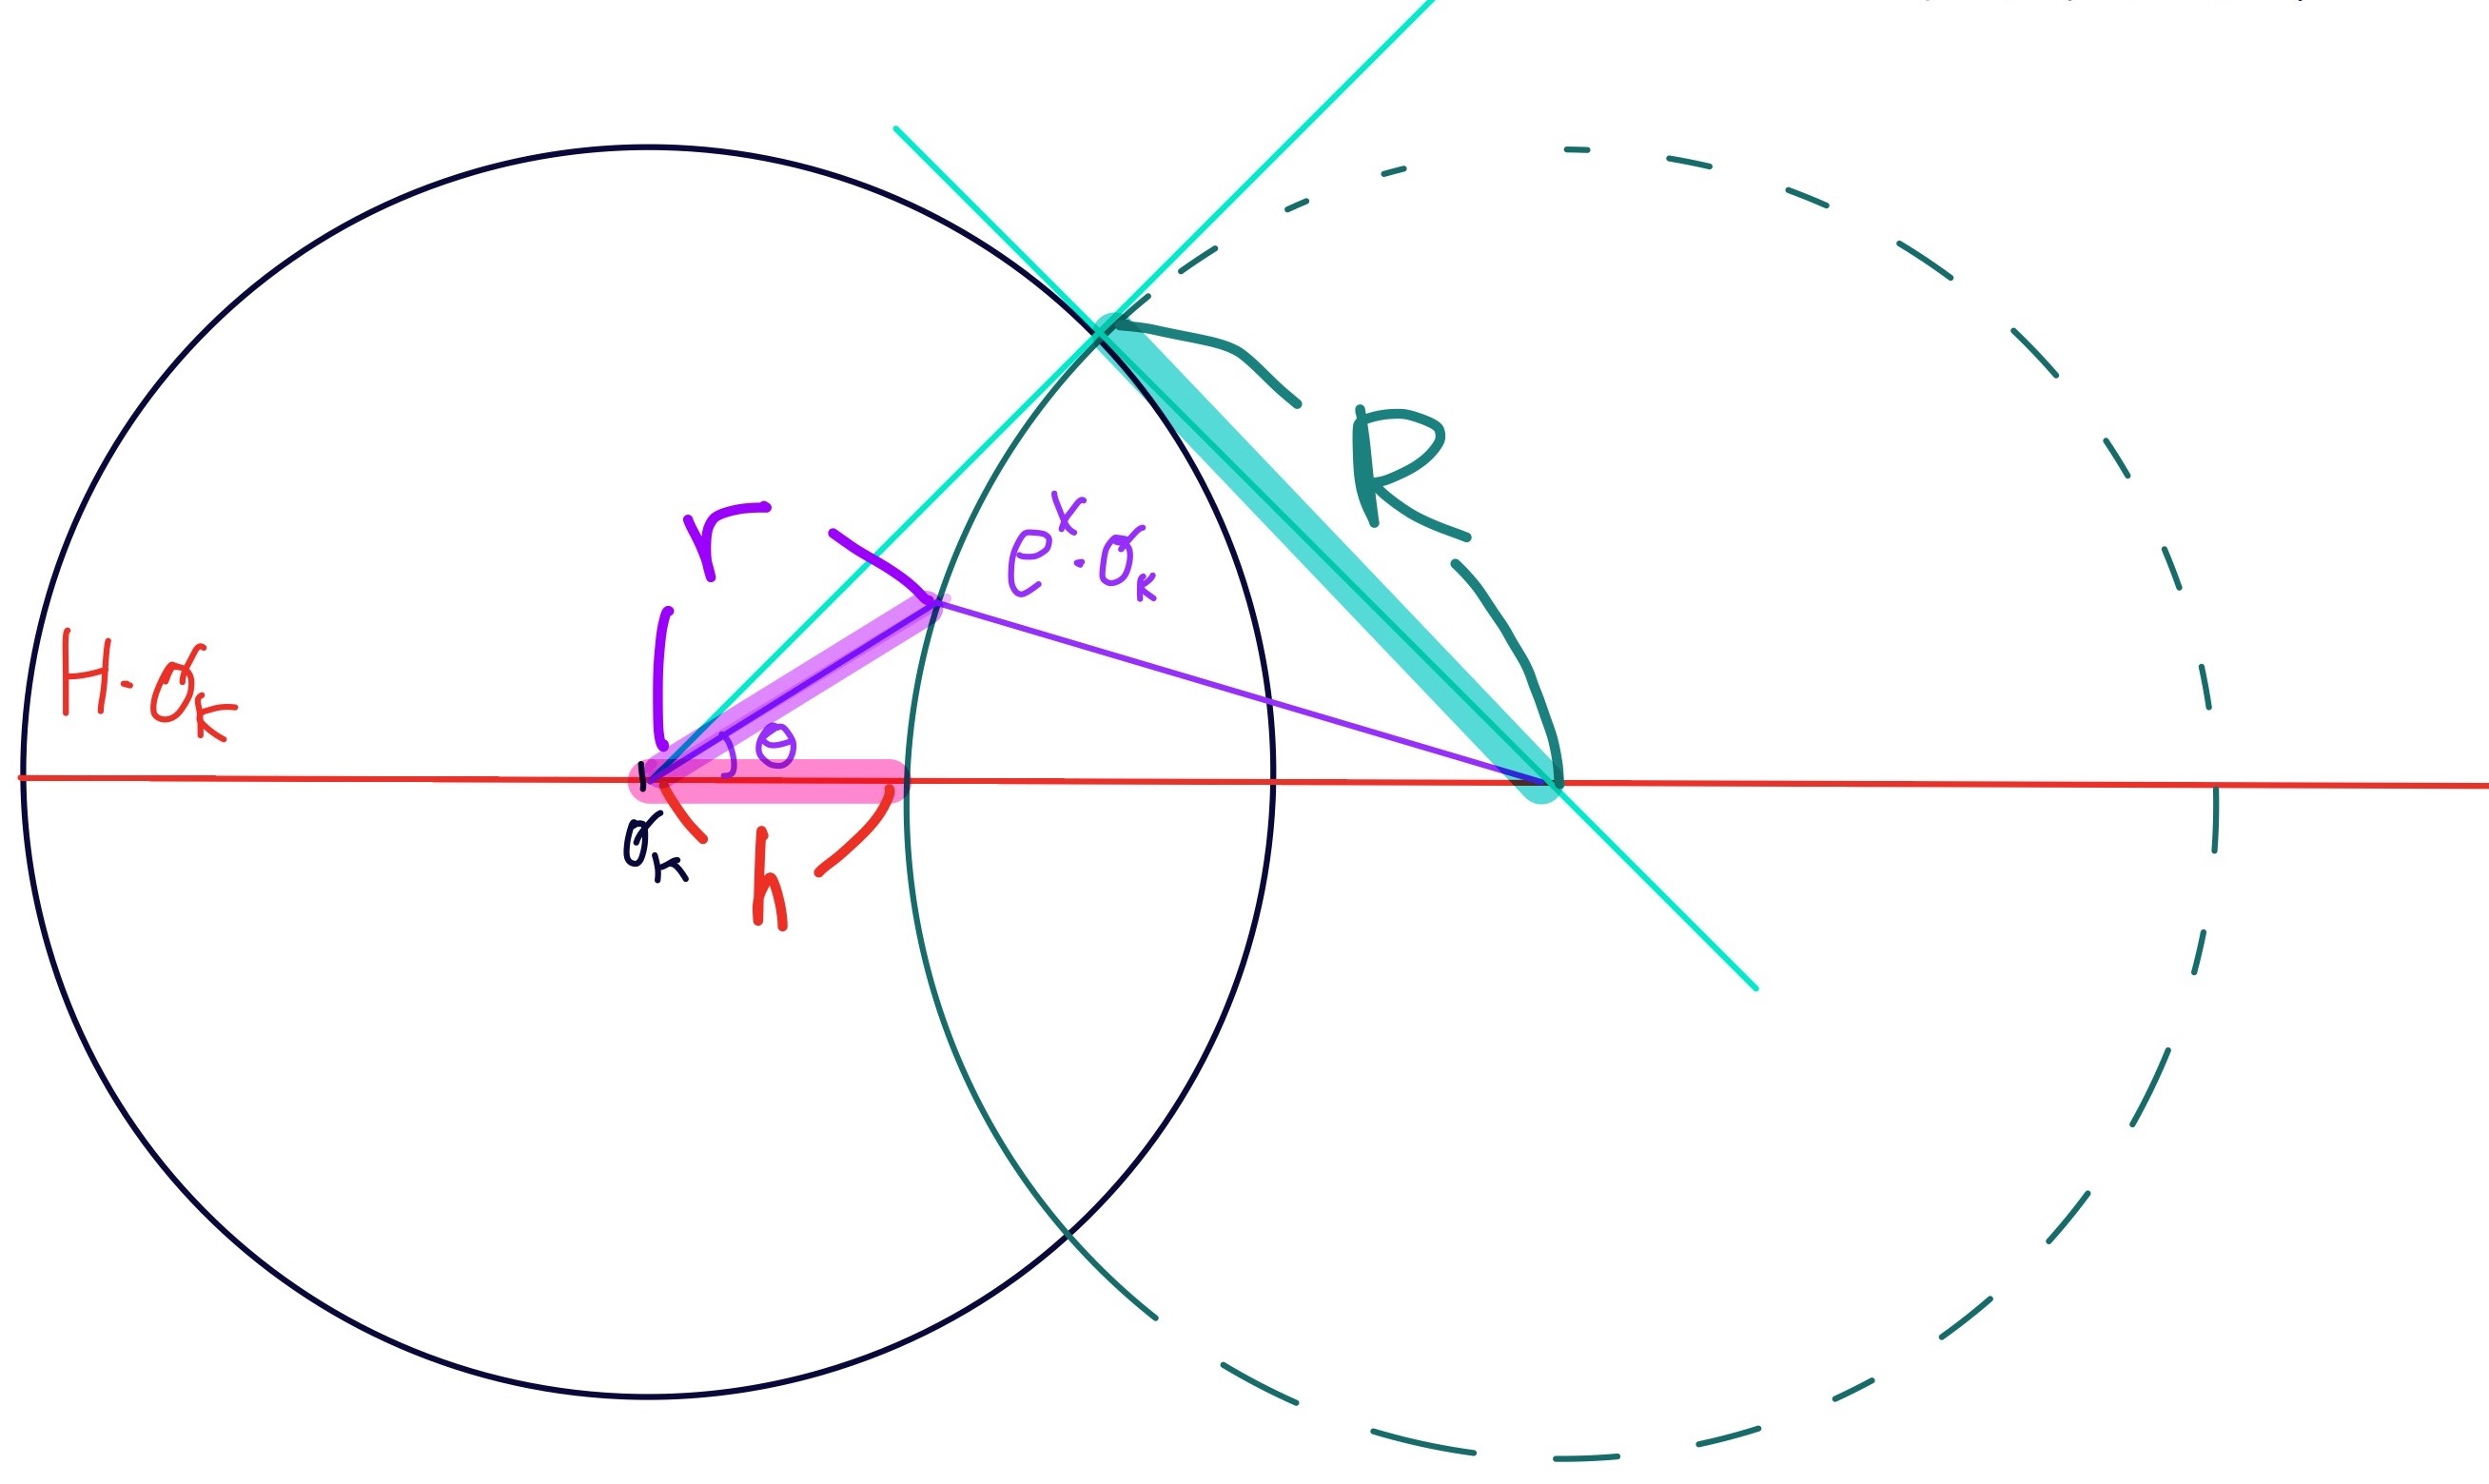
\includegraphics[scale=0.08]{../graph/prob-eg-1.jpg}
    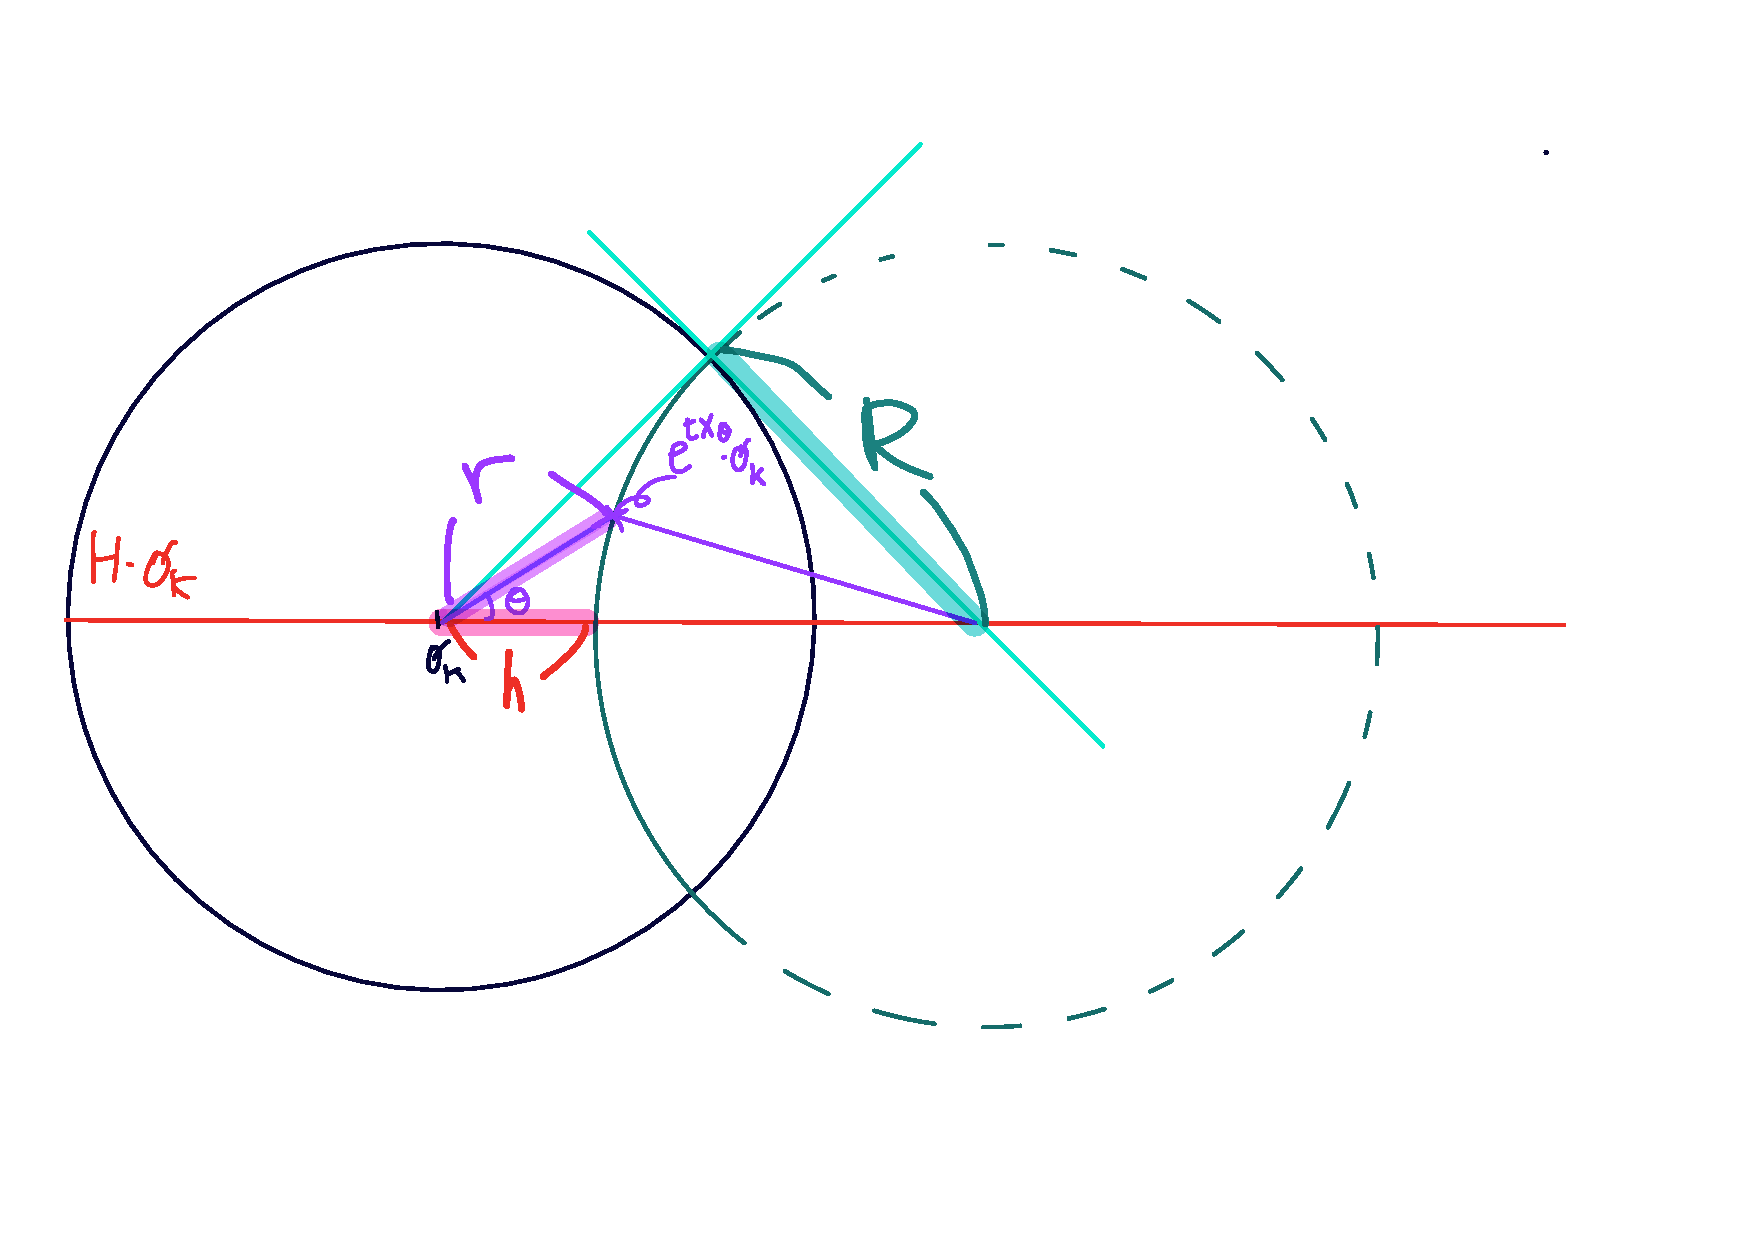
\includegraphics[scale=0.35]{../graph/prob-eg-2.pdf}
    \caption{}
    \label{fig:prob-eg-1}
  \end{figure}

  \Cref{fig:prob-eg-1}では,左の円が{\Poincare}円板$G/K$,右の円は$e^{tX_{\theta}}\cdot o_K $を通り$H\cdot o_K$に垂直に交わる測地線を延長した円を描いた.$G/K$の測地線は境界に直交する円弧であるから,この2つの円は境界で直交している.

  右の円の Euclid 距離での半径を$R$とし,$e^{tX_{\theta}}\cdot o_K $から$H\cdot o_K$への垂線の足の$o_K$からの Euclid 距離を$h$とするとき,外側の青色の直角三角形に対して三平方の定理を用いて$(h+R)^2 = R^2 +  1 $より$R = \dfrac{1-h^2}{2h}$,$R+h = \dfrac{1+h^2}{2h}  $を得る.

  さらに下の紫色の三角形に対して余弦定理を用いて
  \begin{align*}
    {R^2 = (R+h)^2 + r^2 - 2r(R+h)\cos\theta }
  \end{align*}
  を得,
  \begin{align*}
    R^2 &= (R+h)^2 + r^2 - 2(R+h) \cos\theta \\
        &= R^2 +  1 + r^2 - 2r(R+h) \cos\theta \\
        &= R^2 +  1 + r^2 - 2r\dfrac{1+h^2}{2h} \cos\theta  
  \end{align*}
  より
  \begin{align}
    {\dfrac{2r\cos\theta}{r^2 + 1} = \dfrac{2h}{h^2 + 1} }\label{eq:1018-main}
  \end{align}
  を得る.

  $r = \tanh t$,$h = \tanh s$であるから\Cref{eq:1018-main} は$\cos\theta \tanh 2t = \tanh 2t $と書き直せる.したがって$X_{\theta}$に対して$Y(\real X) $が有界であることと$ \abs{\cos\theta}\neq 1 $であること,あるいは$ X\nin \ha  $であることが同値である.
\end{npfwn}

\begin{rem}\label{rem:su11-by-angle}

  \Cref{prop:prob-eg}は角度を用いた議論によっても示すことができる.具体的には,座標を用いた計算により次の\Cref{lem:0106}が示せる (計算は省略する).
  \begin{lem}\label{lem:0106}
    $e^{sY}e^{rZ}\cdot o_K =
    \begin{pmatrix}
      \cosh s & \sinh s\\ \sinh s & \cosh s
    \end{pmatrix}\,
    \sqrt{-1}\tanh r \in \SU(1,1)/\U(1) $,$s > 0$,$r\in \real$に対し,$\phi_{s,r}\defeq \measuredangle_{o_K}(e^{sY}e^{rZ}\cdot o_K,\ e^{sY}\cdot o_K) $は,$\tan \phi_{s,r} = \dfrac{\tanh 2r}{\sinh 2s} $を満たす.ただし$Y \defeq
  \begin{pmatrix}
    0 & 1\\ 1 & 0
  \end{pmatrix}
  $,$Z \defeq \begin{pmatrix}
    0 & \sqrt{-1} \\ -\sqrt{-1} & 0
  \end{pmatrix}$とし,角度$\phi_{s,t} $は$0\leq \phi_{s,r}\leq \frac{\pi}{2} $の範囲に取ることとする.
  \end{lem}  

  \Cref{lem:0106}により\Cref{prop:prob-eg}は次のように証明できる.
  任意の$0\neq s\in \real, r\in \real $に対し,
  \begin{align}
    % \lim_{r\to -\infty}\tan \phi_{\abs{s},r} = \dfrac{-1}{\sinh 2\abs{s}} 
    0 \leq \abs{\tan \phi_{s,r}} \leq  \lim_{r\to \infty}\tan \phi_{\abs{s},r} = \dfrac{1}{\sinh 2\abs{s}}\label{eq:0106}
  \end{align}
  である.$X\nin \real Y $の元に対して$Y(\real X) $が非有界であるとすると,$ 0 <  \epsilon < \phi(X,\ha\cap\pe)$なる$\epsilon$に対し,ある$t\in \real $が存在して,$Y(tX) = s_tY $,$\sinh 2\abs{s_t} > \dfrac{1}{\tan \epsilon} $である.$Z(tX) = r_tZ $とすると\Cref{eq:0106}より$\abs{\tan \phi_{s_t,r_t}} < \tan \epsilon $,したがって
  \begin{align*}
    0\leq \measuredangle_{o_K}(e^{s_tY}e^{r_t Z}\cdot o_K, e^{s_tY}\cdot o_K) < \epsilon < \phi(X,\ha\cap\pe)
  \end{align*}
  となる.しかし定義より$\measuredangle_{o_K}(e^{s_tY}e^{r_t Z}\cdot o_K, e^{s_tY}\cdot o_K) = \measuredangle_{o_K}(e^{tX}\cdot o_K, e^{Y(tX) }\cdot o_K) $であり,$\measuredangle_{o_K}(e^{tX}\cdot o_K, e^{Y(tX) }\cdot o_K) = \phi(X,\ha\cap\pe)$であるから矛盾する. 

  
\end{rem}

\begin{cor}\label{cor:prob-eg}
  $G = \SO(1,n) $,$H = \SO(1,l) $,$1\leq l\leq n-1$は\Cref{prob:1121}の肯定的な例である.具体的には$\pe_{H,\bdd} = \{0\}\cup \pe\setminus\ha $である.% より具体的には次の\Cref{thm:1018-main}が成り立つ.
\end{cor}
% \begin{prop}\label{thm:1018-main}
%   % $\SO(n,1)/\SO(n) $を {\Poincare} ball model で実現したとき,
%   $G = \SO(1,n) $,$H = \SO(1,k) $,$1\leq k\leq n-1$,とする.
%   \begin{align*}
%     Y(X) =
%     \begin{cases}
%       \ds  \frac{1}{4}\inv{\tanh}[\tanh(4\norm{X})\cos\theta ]\frac{X_1}{\norm{X_1}}, &X\in \pe\setminus \per{\ha} \\
%     \ds  0, &X\in  \per{\ha}\cap \pe
%   \end{cases}
%   \end{align*}
%   である.
% \end{prop}
% \begin{cor}
%   % $X\in \pe\setminus \ha $
%   % % $ e^{X}\cdot o_K\nin \SO(k,1)\cdot o_K $
%   % に対し$0 \leq \cos \theta\neq 1$であり,
%   $X\in \pe\setminus\per{\ha}$ならば$0 < \cos \theta \leq 1$であり,
%   \begin{align*}
%     Y(\real X) = \lbig\{s\frac{X_1}{\norm{X_1}} \relmiddle|  -\frac{\inv{\tanh}(\cos\theta)}{4} < s < \frac{\inv{\tanh}(\cos\theta)}{4} \rbig\}
%   \end{align*}
%   であるから,$X\nin \pe_{H,\bdd} $と$X\in \ha\cap \pe $は同値である.したがってこの場合も$\pe_{H,\bdd} =\{0\}\cup\pe\setminus\ha $である.
%   % あるいは$Y(\real X) = \{0\}$ (if $X\in  \per{(\ha)}\cap \pe$) より,$\ha\cap \pe $内で有界である.
% \end{cor}

% \begin{defi}
%   \leavevmode\vspace{-1em}
%   \begin{itemize}
%     \item {\Poincare} ball の計量は$4\dfrac{\sum_i dx_i^2}{(1-x_i^2)^2} $とする.
%     \item $\ds \cos \theta \defeq \frac{\lyama X, \pr(X)\ryama }{\norm{X}\, \norm{\pr(X)}} \geq 0 $,ただし$\lyama{-},{-}\ryama  $は$\solie(n,1) $の Killing 形式とする.
%   \end{itemize} 
% \end{defi}

% \begin{lem}\label{lem:1018}
%   $Z\in \pe$に対し,$e^Z \cdot o_K $が$o_K$から Euclid 距離で$\tanh p$,$p \geq 0$の位置にある場合,$\norm{Z} = \frac{p}{2} $である.
% \end{lem}



\begin{skpfwn}{\Cref{cor:prob-eg}}% \bluetext{make it precise}
  $\SO(1,n) $の$\real^{n+1} $への自然表現を用いて$\SO(1,n)/\SO(n)\simeq \{\trans{(x_1\cldots x_n)} \in \real^n \mid \sum_{1\leq i\leq n}x^2_i  < 1 \} $として実現する (後述する\Cref{nttdef:1127-main}と同様).この実現において$\SO(1,l)/\SO(n)\cap\SO(1,l) \simeq \{\trans{(x_1\cldots x_n)}\in \real^n \mid x_{l+1} = \cdots = x_n = 0 \text{ かつ } \sum_{1\leq i\leq n}x^2_i  < 1 \} $である.

  \Cref{lem:1101}より$X$を任意の$k\in K$で$\Ad(k)\ha = \ha $なる$k$に対し$\Ad(k) X$に取り替えて$Y(\real X) $の有界性を議論して一般性を失わないから,$k\in \SO(1,l)\cap\SO(n) $を適当に取ることにより
  \begin{align}
    X =
    \begin{pmatrix}
      0 & p_1 & 0 & \cdots & 0 & p_{l+1} & \cdots & p_{n}\\
      p_1 &  &  &  &  &  &  \\
      0 &  &  &  &  &  &  \\
      \vdots &  &  &  &  &  &  \\
      0&  &  &  &  &  &  \\
      p_{l+1}  &  &  &  &  &  &  \\
      \vdots &  &  &  &  &  &  \\
      p_{n}  &  &  &  &  &  &  \\
    \end{pmatrix} \label{eq:X-1}
  \end{align}
  (空白部分はすべて0) としてよい.さらに適当な$A\in \SO(n-l) $に対し,
  \begin{align*}
     \left(
    \begin{array}{cccc|cc}
      &&&&&\\     
      &&&&&\\
      &\mbox{\smash{\huge $I_{l+1}$}}&&&&\\
      &&&&&\\     
      &&&&\\ \hline
      &&&&\\
      &&&&&\mbox{\smash{\huge $A$}}\\
      &&&&&
    \end{array}
               \right)
  \end{align*}
  (空白部分はすべて0) を\Cref{eq:X-1}の$X$に作用させることにより$X$の形を
  \begin{align}
    X =
    \begin{pmatrix}
      0 & p_1 & 0 & \cdots & 0 & p_{l+1} &0  & \cdots & 0\\
      p_1 &  &  &  &  &  &  \\
      0 &  &  &  &  &  &  \\
      \vdots &  &  &  &  &  &  \\
      0&  &  &  &  &  &  \\
      p_{l+1}  &  &  &  &  &  &  \\
      0  &  &  &  &  &  &  \\
      \vdots &  &  &  &  &  &  \\
      0  &  &  &  &  &  &  \\
    \end{pmatrix} \label{eq:X-1}
  \end{align}
  と仮定して良い.

  このときある$q_1,q_{l+1}\cldots q_{n}\in \real$によって$e^{X}\cdot o_K \in \SO(1,n)/\SO(n) $は$ \trans{( q_1,0\cldots 0, q_{l+1}\cldots q_{n})} $に対応する.
  

  $\trans{(q_1,0\cldots 0, q_{l+1}\cldots q_{n})} $と$\trans{(0\cldots 0)} $を結ぶ直線と$ \trans{(q_1,0\cldots 0)}$と$\trans{(0\cldots 0)}$を結ぶ直線で張られる2次元平面で$\SO(1,n)/\SO(n)$を切った際の断面を考える.
  \begin{figure}[H]
    \centering
    % \raggedleft
    % \raggedrightp
    % \includegraphics[scale=0.08]{../graph/fig1.jpg}
    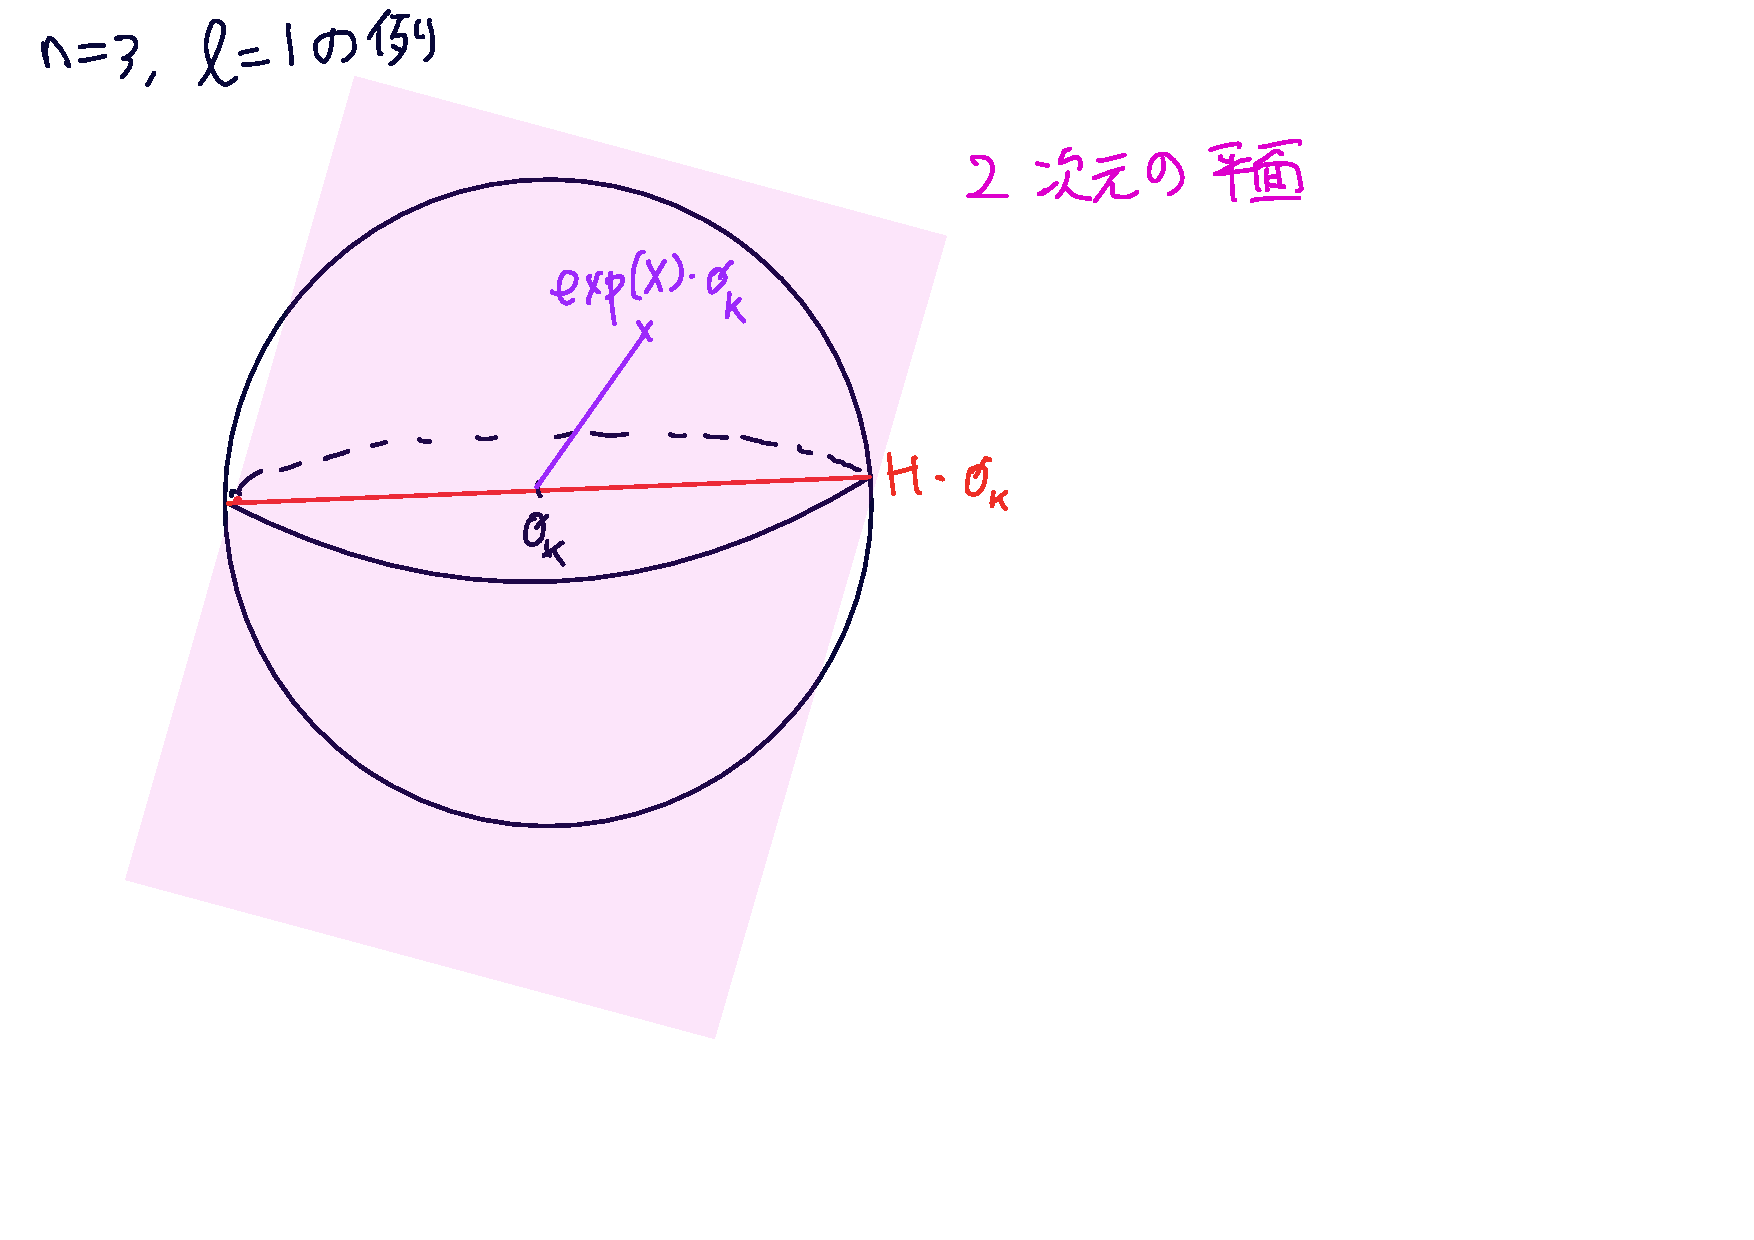
\includegraphics[scale=0.4]{../graph/son1-5.pdf}
    \caption{}
    \label{fig:son1}
  \end{figure}
  
  この断面に現れるのは\Cref{fig:prob-eg-1}と同様の{\Poincare}円板 (Riemann計量は定数倍で変わりうる) であるから,同様の計算により\Cref{cor:prob-eg}を得る.

  % よって\Cref{lem:1018}より,$\norm{Y(X)} = \frac{s}{2} = \frac{1}{4}\inv{\tanh}(\cos\theta \tanh 2t) $を得る.再び\Cref{lem:1018}より$4\norm{X} = 2t $であるから,$\norm{Y(X)} = \frac{1}{4}\inv{\tanh}[\tanh(4\norm{X})\cos\theta] $を得,\Cref{thm:1018-main}の主張が従う.  
\end{skpfwn}


\subsection{\Cref{prob:1121}の観察: \Cref{prob:1121}の条件が落とせないことを示すいくつかの例}

\Cref{lem:basic-prob}より\Cref{prob:1121}は$G$の実階数が1の場合には次の問と同値であった.
\begin{q}\label{prob:1121-2}

  \begin{align}
    \pe_{H,\bdd} &= \{0\}\cup \pe\setminus\ha\notag \\
                 &= \{X\in \pe\mid [X_1, X_2]\neq 0 \text{ あるいは } X\in \per{\ha}\cap\pe \text{ である.}  \}\label{eq:prob-1121-2}\\
                 &= \{X\in \pe\mid [X, (\ha\cap \pe)]\neq 0 \text{ あるいは } X\in \per{\ha}\cap\pe \text{ である.}  \}\label{eq:prob-1121-3}
  \end{align}
  となるか?  
\end{q}

ここで$G$の実階数が2の場合には一般的には\Cref{eq:prob-1121-2}は成り立たないことがわかっている.
\begin{prop}\label{prop:0114}
  $G = \SL(3,\real) $,$H = \{\diag(e^a,e^b,e^c)\mid a,b,c\in \real,\ a+ b + c = 0 \} $,$X\defeq
  \begin{pmatrix}
    1 & 0 & 0 \\
    0 & 0 & \sqrt{2} \\
    0 & \sqrt{2} & -1
  \end{pmatrix}
  $に対し$Y(\real X) $は非有界である.
\end{prop}


$\ha = \{\diag(a,b,c)\mid a,b,c\in \real,\ a +b + c = 0 \}  $であるから$X_1 = \diag(1,0,-1)$,$X_2 = \begin{pmatrix}
  0 & 0 & 0 \\
  0 & 0 & \sqrt{2} \\
  0 & \sqrt{2} & 0
\end{pmatrix}$であり,$[X_1, X_2] = \begin{pmatrix}
  0 & 0 & 0 \\
  0 & 0 & \sqrt{2} \\
  0 & -\sqrt{2} & 0
\end{pmatrix} \neq 0$より$X$は\Cref{eq:prob-1121}の右辺の集合の元ではあるが$X\nin \pe_{H,\bdd} $であるから,\Cref{prop:0114}は\Cref{prob:1121}の反例となっている.

1つ補題を用意してから\Cref{prop:0114}を証明する.
\begin{lem}\label{lem:0114}
  任意の$t\in \real$に対し
  \begin{align*}
    \exp\lbig(2t\begin{pmatrix}
      0 & \sqrt{2} \\
      \sqrt{2} & -1 
    \end{pmatrix}\rbig) &=
                 \begin{pmatrix}
                   \dfrac{2e^{2t} + e^{-4t}}{3} &  \dfrac{\sqrt{2} (e^{2t} - e^{-4t})}{3}\\
                   \\
                   \dfrac{\sqrt{2} (e^{2t} - e^{-4t})}{3} & \dfrac{e^{2t} + 2e^{-4t}}{3}
                 \end{pmatrix}
  \end{align*}
  である.
\end{lem}

\begin{npfwn}[\Cref{lem:0114}]

  $ \theta $を$\cos 2\theta = \dfrac{1}{3} $,$\sin 2\theta = \dfrac{-2\sqrt{2}}{3} $を満たす実数として任意に1つ固定する.このとき
  \begin{align*}
    \cos^2 \theta &= \dfrac{1 +\cos 2\theta}{2} = \dfrac{2}{3},\\
    \sin^2 \theta &= \dfrac{1-\cos 2\theta}{2} = \dfrac{1}{3}
  \end{align*}
  である.$k \defeq
  \begin{pmatrix}
    \cos \theta & -\sin \theta \\ \sin \theta & \cos \theta
  \end{pmatrix}
  $とすると,
  \begin{align*}
    k
    \begin{pmatrix}
      0 & \sqrt{2} \\
      \sqrt{2} & -1 
    \end{pmatrix}\inv{k} &=
                           \begin{pmatrix}
                             -2\sqrt{2}\sin\theta \cos\theta  - \sin^2\theta & \sqrt{2}(\cos^2 \theta - \sin^2\theta) + \cos\theta \sin\theta \\
                             \sqrt{2}(\cos^2 \theta - \sin^2\theta) + \cos\theta \sin\theta  & 2\sqrt{2}\sin\theta \cos\theta  - \cos^2\theta
                           \end{pmatrix}\\
        &=
          \begin{pmatrix}
            -\sqrt{2}\sin 2\theta  - \sin^2\theta & \sqrt{2}\cos 2\theta + \dfrac{\sin 2\theta}{2} \\
            \sqrt{2}\cos 2\theta + \dfrac{\sin 2\theta}{2}  &\sqrt{2}\sin 2 \theta - \cos^2\theta
          \end{pmatrix}\\
        &=
          \begin{pmatrix}
            1  &  0\\ 0 & -2
          \end{pmatrix}
  \end{align*}
  である.

  したがって
  \begin{align*}
    k\exp\lbig(2t\begin{pmatrix}
      0 & \sqrt{2} \\
      \sqrt{2} & -1 
    \end{pmatrix}\rbig)\inv{k} &= \exp
                                 \begin{pmatrix}
                                   2t & 0 \\ 0 & -4t
                                 \end{pmatrix}
  \end{align*}
  であるから,
  \begin{align*}
    \exp\lbig(2t\begin{pmatrix}
      0 & \sqrt{2} \\
      \sqrt{2} & -1 
    \end{pmatrix}\rbig) &= \inv{k} \exp\lbig(
                                 \begin{pmatrix}
                                   2t & 0 \\ 0 & -4t
                                 \end{pmatrix}\rbig)k\\
        &=
          \begin{pmatrix}
            \cos \theta  & \sin \theta \\ -\sin \theta & \cos \theta
          \end{pmatrix}
                                                         \begin{pmatrix}
                                                           e^{2t} & 0 \\ 0 & e^{-4t}
                                                         \end{pmatrix}
                                                                             \begin{pmatrix}
                                                                               \cos \theta  & -\sin \theta \\ \sin \theta & \cos \theta
                                                                             \end{pmatrix}\\
        &=
          \begin{pmatrix}
            e^{2t}\cos^2\theta + e^{-4t}\sin^2 \theta  & (e^{-4t} - e^{2t})\sin\theta \cos\theta \\ (e^{-4t} - e^{2t})\sin\theta \cos\theta  & e^{2t}\sin^2\theta +e^{-4t}\cos^2\theta
          \end{pmatrix}\\
        &= \begin{pmatrix}
          \dfrac{2e^{2t} + e^{-4t}}{3} &  \dfrac{\sqrt{2} (e^{2t} - e^{-4t})}{3}\\
          \\
          \dfrac{\sqrt{2} (e^{2t} - e^{-4t})}{3} & \dfrac{e^{2t} + 2e^{-4t}}{3}
                 \end{pmatrix}
  \end{align*}
\end{npfwn}

\begin{npfwn}[\Cref{prop:0114}]
  行列式1の$3\times 3$正定値実対称行列全体の集合$\Symm^{+}(3)$と$G/K$は$gK \mapsto g
  \begin{pmatrix}
    1 & 0\\ 0 & 1
  \end{pmatrix}
  \trans{g} $により微分同相である.
  
  \Cref{lem:0114}より
  \begin{align}
    e^{tX}\cdot o_K &= e^{tX}\; \trans{(e^{tX})} = e^{2tX}\notag\\
                    &= \begin{pmatrix}
                      e^{2t} & 0 & 0 \\
                      0 & \dfrac{2e^{2t} + e^{-4t}}{3} &  \dfrac{\sqrt{2} (e^{2t} - e^{-4t})}{3}\\
                      % \\
                      0 & \dfrac{\sqrt{2} (e^{2t} - e^{-4t})}{3} & \dfrac{e^{2t} + 2e^{-4t}}{3}
                    \end{pmatrix}\label{eq:0114-1}
  \end{align}
  である.

  $Y \defeq \diag(a,b,c)  $,$a + b + c = 0$,$Z \defeq
  \begin{pmatrix}
    0 & 0 & 0\\
    0 & 0 & 1\\
    0 & 1 & 0
  \end{pmatrix}
  $とすると,$r\in \real$に対し,
  \begin{align}
    e^{Y}e^{rZ}\cdot o_K &= e^{Y}e^{2rZ}e^{Y}\notag\\
                         &=
                           \begin{pmatrix}
                             e^{a} & 0 & 0 \\
                             0 & e^{b} & 0\\
                             0 & 0 & e^{c}
                           \end{pmatrix}
                                     \begin{pmatrix}
                                       1 & 0 & 0\\
                                       0 & \cosh 2r & \sinh 2r \\
                                       0 & \sinh 2r & \cosh 2r
                                     \end{pmatrix}
                                                      \begin{pmatrix}
                                                        e^{a} & 0 & 0 \\
                                                        0 & e^{b} & 0\\
                                                        0 & 0 & e^{c}
                                                      \end{pmatrix}\notag\\
                         &=
                           \begin{pmatrix}
                             e^{2a} & 0 & 0\\
                             0 & e^{2b}\cosh 2r & e^{b+c}\sinh 2r \\
                             0 & e^{b+c}\sinh 2r & e^{2c}\cosh 2r
                           \end{pmatrix}\notag\\
                         &= \begin{pmatrix}
                             e^{2a} & 0 & 0\\
                             0 & e^{2b}\cosh 2r & e^{-a}\sinh 2r \\
                             0 & e^{-a}\sinh 2r & e^{-2a-2b}\cosh 2r
                           \end{pmatrix}\label{eq:0114-2}
  \end{align}
  である.ただし最後の変形には$a + b + c = 0$を用いた.

  \Cref{eq:0114-1}と\Cref{eq:0114-2}を見比べると,
  \begin{align*}
    a &= t,\\
    \sinh 2r &= \dfrac{2\sqrt{2}}{3}\sinh 3t, \\
    e^{2b} &= \dfrac{2e^{2t} + e^{-4t}}{\sqrt{9 + 8\sinh^2 3t}}
  \end{align*}
  とすると$e^{Y}e^{rZ}\cdot o_K = e^{tX}\cdot o_K $を得る.つまり任意の$t\in \real$に対し
  \begin{itemize}
  \item $Y(tX) = \diag(a(t) ,b(t) ,-a(t) -b(t) ) $

    ただし$a(t) = t$,$b(t) =\dfrac{1}{2} \log \lbig(\dfrac{2e^{2t} + e^{-4t}}{\sqrt{9 + 8\sinh^2 3t}}\rbig) $,
  \item $Z(tX) = r(t)Z  $ただし$r(t) = \dfrac{1}{2} \inv{\sinh}\lbig( \dfrac{2\sqrt{2}}{3}\sinh 3t\rbig) $
  \end{itemize}
  であるから,$Y(\real X) $は非有界である.  
\end{npfwn}



$G$が実階数1の場合に限っても\Cref{prob:1121-2}と類似の問題はいくつか考えられる.例えば\Cref{eq:prob-1121-3}において$\ha\cap\pe$を$\ha$に置き換えた次の問が立てられる.
\begin{q}\label{prob:1101}
  $\pe_{H,\bdd} = \{X\in \pe\mid  [X,\ha]\neq \{0\} \text{ あるいは } X\perp \ha \text{ である.}\}  $となるか?
\end{q}

しかし\Cref{prob:1101}にも主張が成り立たない実階数2の例が存在する.
\begin{lem}\label{lem:1118-main}
  $G = \SL(3,\real) $,$Y_1\defeq \diag(1,1,-2)$,$Y_2 \defeq \begin{pmatrix}
    0 & 1 & 0\\
    -1 & 0 & 0 \\
    0 & 0 & 0
  \end{pmatrix}$,\\
  $\ha = \real Y_1 \oplus \real Y_2 $,$X = \diag(1,0,-1) $に対し,$[X,\ha] \neq \{0\} $であるが$Y(\real X) = \real Y_1 $であり,非有界である.
\end{lem}

\begin{npfwn}[\Cref{lem:1118-main}]

  $\ha$は可換Lie環であり,$\ge = \slie(3,\real) $のCartan対合$\theta W \defeq -\trans{W} $に対し$\ha = \theta \ha$である.

  $[X,\ha]\neq \{0\} $は,$[X, Y_2] \neq 0$より従う.

  ここで$Z_1\defeq \diag(1,-1,0)\in \per{\ha}\cap \pe $であり,任意の$t\in \real$に対し,$e^{2tX} = e^{tY_1}e^{tZ_1} $であるから,$Y(\real X) = \real Y_1 $となり,\Cref{lem:1118-main} が示された.
\end{npfwn}

\Cref{lem:1118-main}において$X$と$\ha$は,$[X,\ha] \neq \{0\} $だが$[X,(\ha\cap \pe)] = \{0\}$かつ$X\not\perp (\ha\cap \pe) $となるように取った.したがって\Cref{prob:1101}の右辺を次の\Cref{prob:1101-2}のように少し弱めても\Cref{lem:1118-main}は\Cref{prob:1101-2}が成り立たないような例になっている.
\begin{q}\label{prob:1101-2}
  $\pe_{H,\bdd} = \{X\in \pe\mid  [X,\ha]\neq \{0\} \text{ あるいは } X\perp (\ha\cap\pe) \text{ である.} \}  $となるか?
\end{q}
